\documentclass[12pt, oneside]{book}
\usepackage[a4paper,top=2.5cm,bottom=2.5cm,left=3.5cm,right=2cm]{geometry}
\usepackage[utf8]{inputenc}
\usepackage[T1]{fontenc}
\usepackage{graphicx}
\usepackage{url}
\usepackage[english]{babel} % vypnite pre prace v anglictine
\usepackage{color}
\usepackage{stmaryrd}
\usepackage{amsmath} 
\usepackage{amsthm}
\usepackage{listings}
\usepackage{caption}
\usepackage{subcaption}
\usepackage{float}
\usepackage[final]{pdfpages}
%\usepackage[none]{hyphenat}
\usepackage{algorithm2e}
\usepackage{hyperref}
\usepackage{booktabs}
\usepackage{indentfirst}
\usepackage{enumerate}
\usepackage{enumitem}

%\usepackage{epigraph}

\usepackage{nameref}


\definecolor{lightgray}{gray}{0.9}
\lstset{
    showstringspaces=false,
    basicstyle=\ttfamily,
    keywordstyle=\color{blue},
    commentstyle=\color[grey]{0.6},
    stringstyle=\color[RGB]{255,150,75}
}

\newcommand{\inlinecode}[2]{\colorbox{lightgray}{\lstinline[language=#1]$#2$}}

\DeclareCaptionType{equ}[][]

\lstset{
        mathescape=true,
        literate=
               {=}{$\leftarrow{}$}{1}
               {==}{$={}$}{1},
        morekeywords={if,then,else,return,for,def}
        }


\theoremstyle{definition}
\newtheorem{definition}{Definition}[section]


\linespread{1.25} % hodnota 1.25 by mala zodpovedat 1.5 riadkovaniu
\setcounter{secnumdepth}{3}

% -------------------
% --- Definicia zakladnych pojmov
% --- Vyplnte podla vasho zadania
% -------------------
\def\mfrok{2018}
\def\mfnazov{Improving LSA word weights for document classification}
\def\mftyp{master's thesis}
\def\mfautor{Bc. Vladimír Macko}
\def\mfskolitel{RNDr. Kristína Malinovská, PhD.}
\def\*{{\color{red} \bf FIXME: }}

%ak mate konzultanta, odkomentujte aj jeho meno na titulnom liste
\def\mfkonzultant{RNDr. Radim Řehůřek, PhD.}  

\def\mfmiesto{Bratislava, \mfrok}

%aj cislo odboru je povinne a je podla studijneho odboru autora prace
\def\mfodbor{ Informatics } 
\def\program{ Informatics }
\def\mfpracovisko{ Department of Computer Science }

\newcommand{\specialcell}[2][c]{%
  \begin{tabular}[#1]{@{}l@{}}#2\end{tabular}}

\begin{document}     

% -------------------
% --- Obalka ------
% -------------------
\thispagestyle{empty}

\begin{center}
\sc\large
COMENIUS UNIVERSITY, BRATISLAVA\\
FACULTY OF MATHEMATICS, PHYSICS AND INFORMATICS

\vfill

{\LARGE\mfnazov}\\
\mftyp
\end{center}

\vfill

{\sc\large 
\noindent \mfrok\\
\mfautor
}

\eject % EOP i
% --- koniec obalky ----

% -------------------
% --- Titulný list
% -------------------

\thispagestyle{empty}
\noindent

\begin{center}
\sc  
\large
COMENIUS UNIVERSITY, BRATISLAVA\\
FACULTY OF MATHEMATICS, PHYSICS AND INFORMATICS

\vfill

{\LARGE\mfnazov}\\
\mftyp
\end{center}

\vfill

\noindent
\begin{tabular}{ll}
Study programme: & \program \\
Study field: & \mfodbor \\
Department: & \mfpracovisko \\
Supervisor: & \mfskolitel \\
Consultant: & \mfkonzultant \\
\end{tabular}

\vfill


\noindent \mfmiesto\\
\mfautor

\eject % EOP i


% --- Koniec titulnej strany


% -------------------
% --- Zadanie z AIS
% -------------------
% v tlačenej verzii s podpismi zainteresovaných osôb.
% v elektronickej verzii sa zverejňuje zadanie bez podpisov

\newpage 
\thispagestyle{empty}
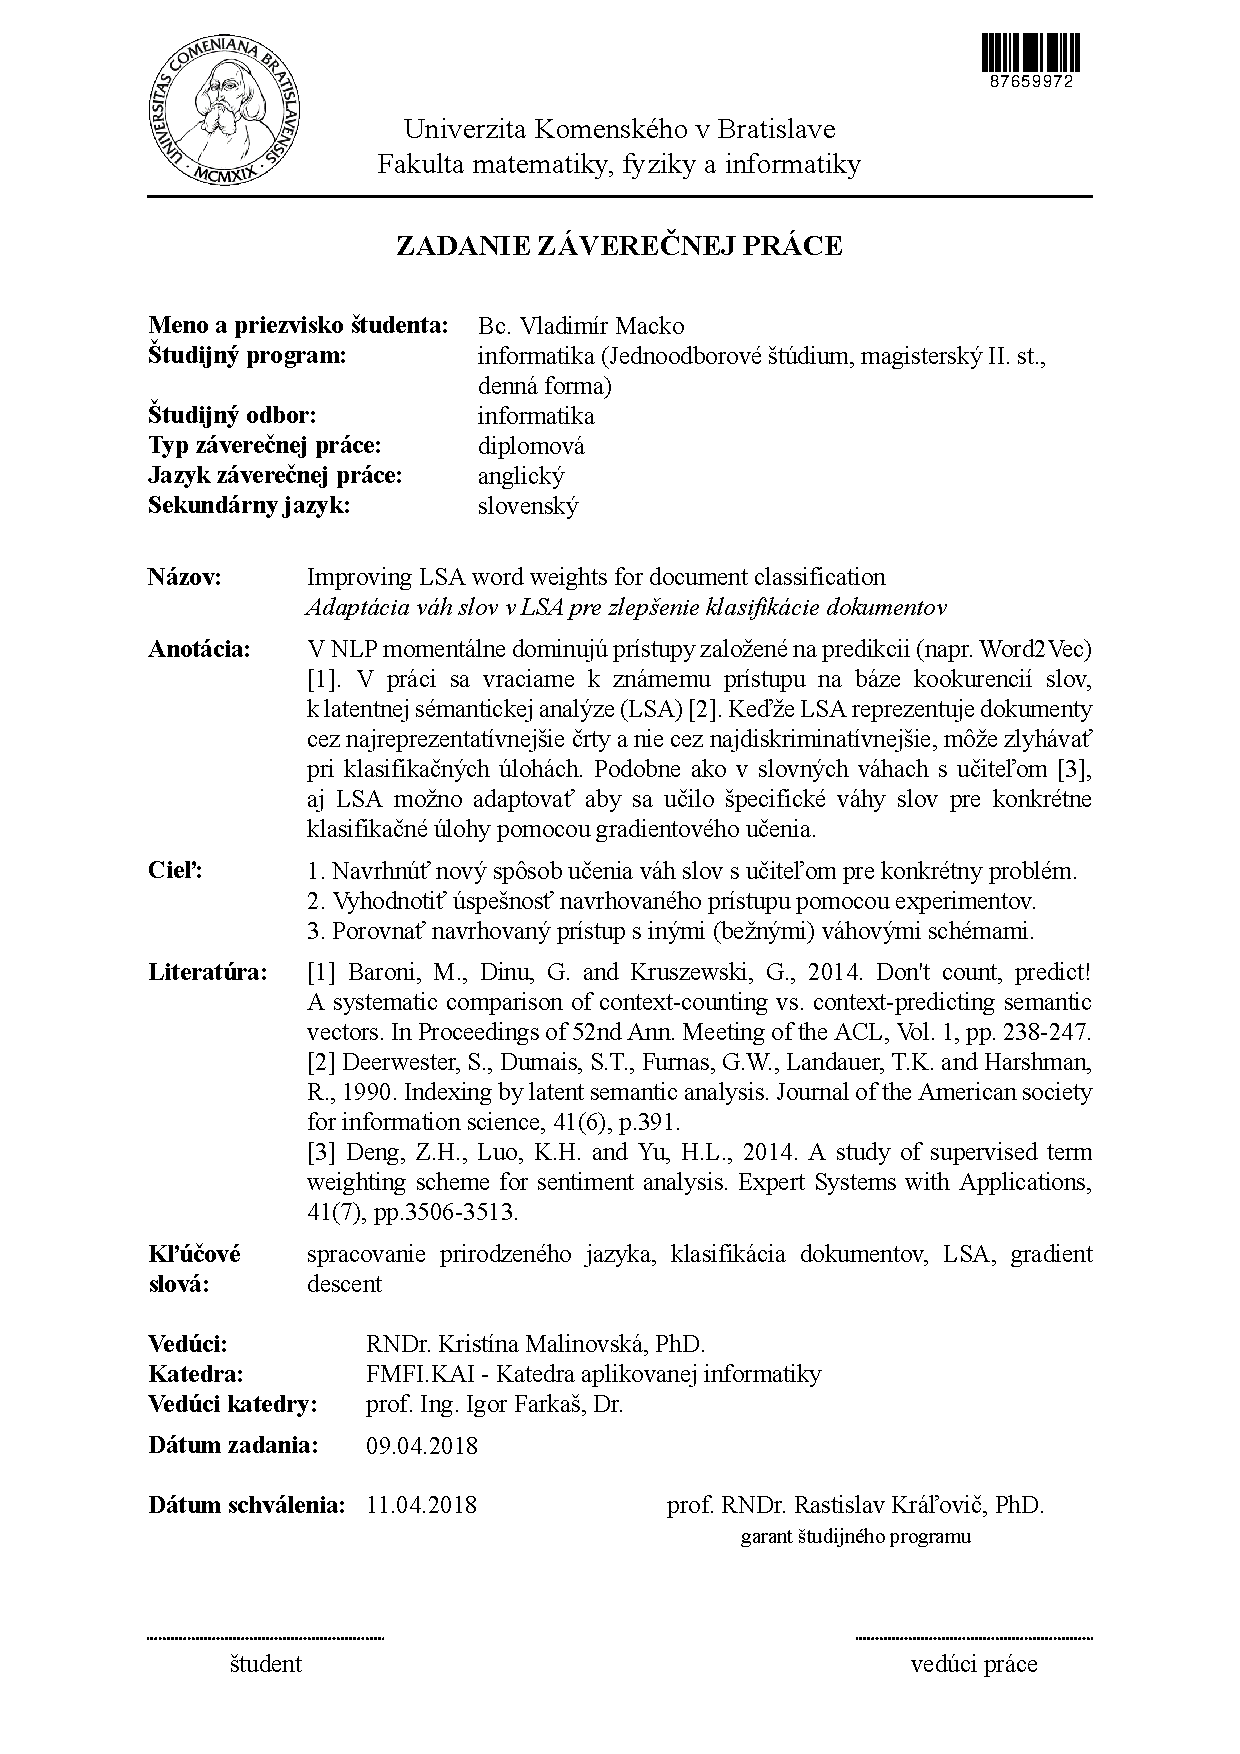
\includepdf[pages={1}]{misc/vmacko-zadanie-sk.PDF}

\newpage 
\thispagestyle{empty}
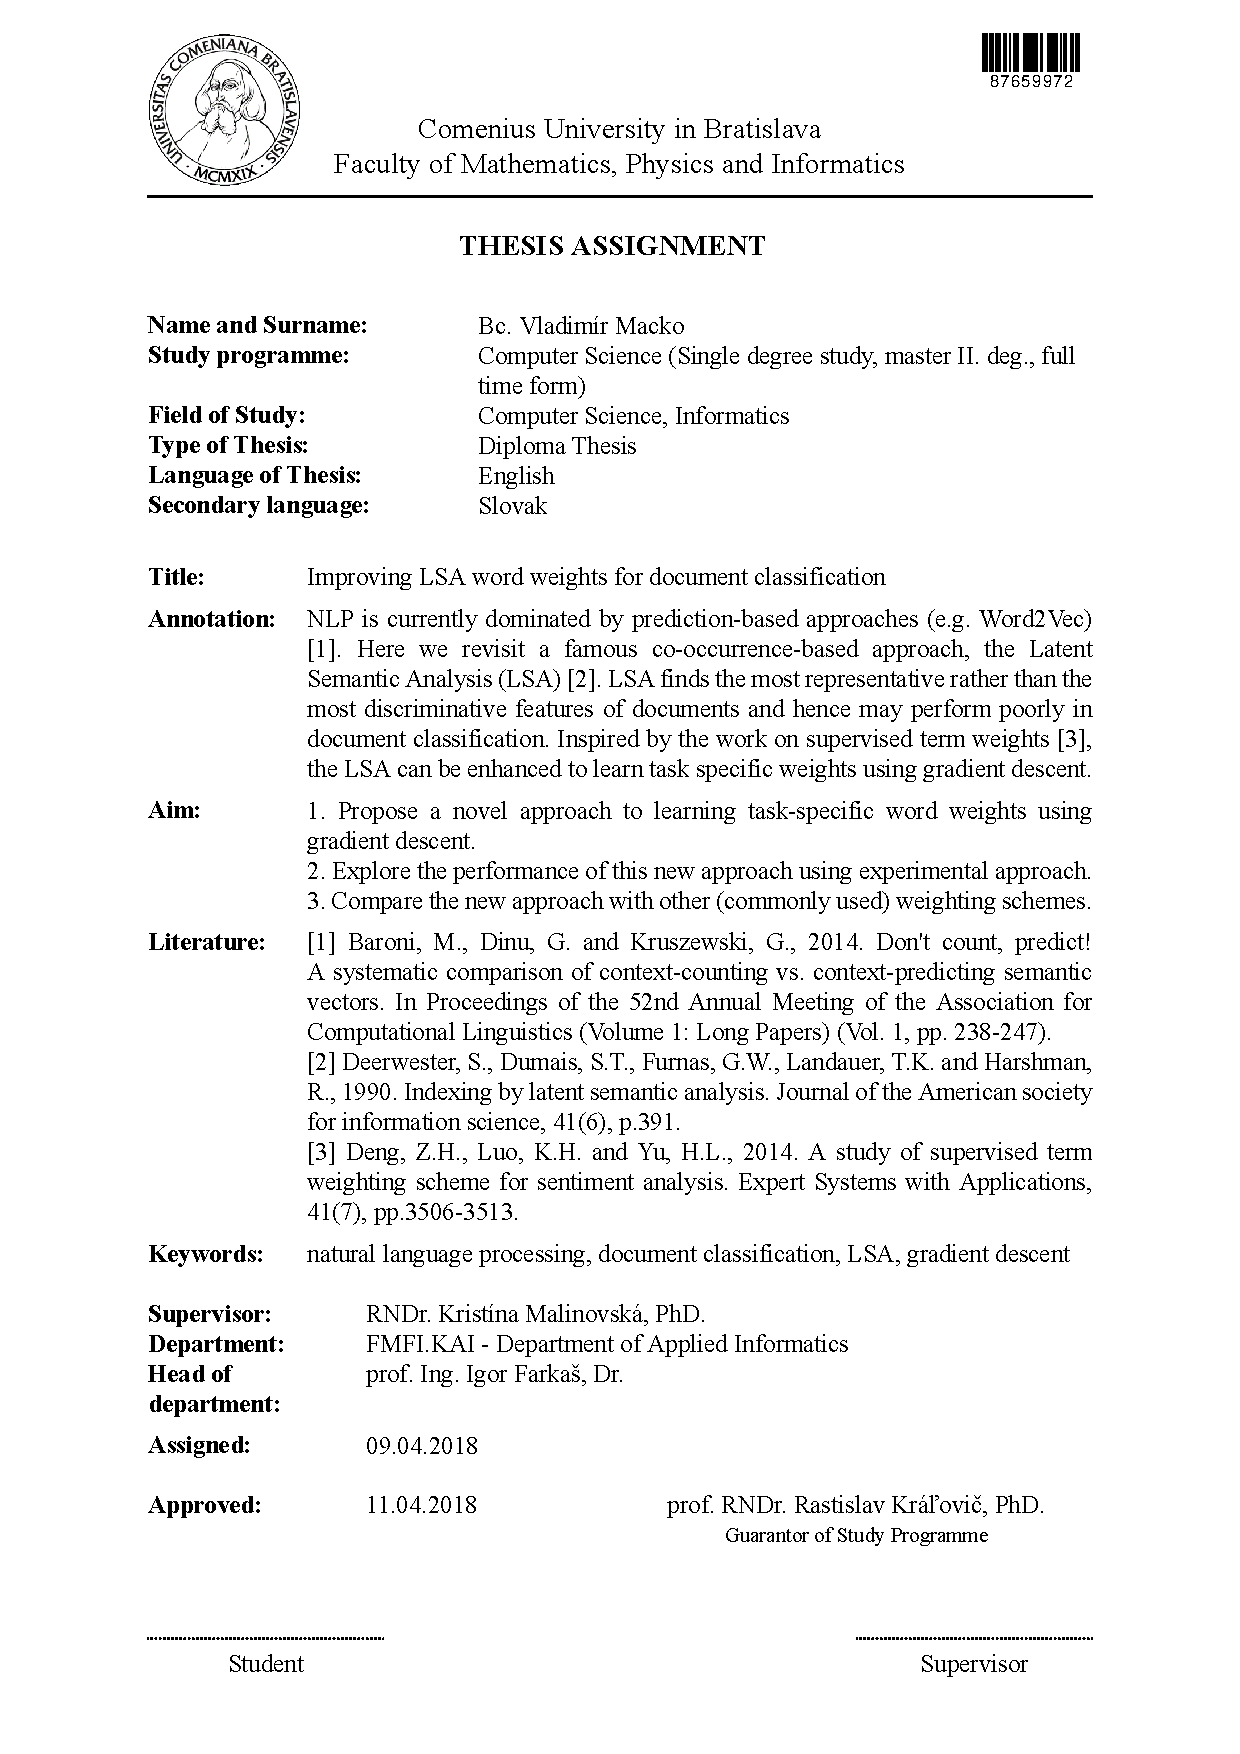
\includepdf[pages={1}]{misc/vmacko-zadanie-en.PDF}

% --- Koniec zadania

\frontmatter

% -------------------
%   Poďakovanie - nepovinné
% -------------------
\setcounter{page}{3}
\newpage 
~

\vfill
{\bf Acknowledgment:} 
I would like to thank my supervisor Kristina Malinovská, for complementing my writing weaknesses. 
Also, I would like to thank my colleagues from CEAI, where I learned tons of invaluable research and programming skills, without which I would not be able to properly finish this thesis.
Special thanks go to Radim Řehůřek, who responded to an email of a random guy (me), who asked him for mentoring and advice.
I would also like to express my gratitude to Majka, for valuable suggestions and for her own thesis, which provided me with literary inspirations.
Next, I want to thank Guido van Rossum, for creating a tool, which inflicted to me the most pain and caused the most professional joy in my life. 
Last, but not least, huge thanks goes to Baša, my family, and my friends for supporting me in this funny period of time. 
% --- Koniec poďakovania




% -------------------
%   Abstrakt - Slovensky
% -------------------
\newpage 
\section*{Abstrakt}

Latentná sémantická analýza môže zlyhávať pri klasifikačných úlohách, lebo vyberá črty dokumentov, ktoré sú najreprezentatívnejšie, ale nie najdiskriminatívnejšie. 
V~tejto práci predstavujeme novú metódu eLSA, ktorá prináša ďalšiu vrstvu váh $w'$, ktoré sú trénované pomocou metódy najväčšieho vzostupu.
Experimentálne sme ukázali, že proces učenia eLSA konverguje, a že eLSA dosahuje väčšiu presnosť ako LSA.
Taktiež využívame eLSA na analyzovanie bežne používaných váhových schém a identifikujeme slová, ktoré tieto schémy podhodnocujú alebo nadhodnocujú.

\paragraph*{Kľúčové slová:} spracovanie prirodzeného jazyka, klasifikácia dokumentov, gradient descent, LSA
% --- Koniec Abstrakt - Slovensky


% -------------------
% --- Abstrakt - Anglicky 
% -------------------
\newpage 
\section*{Abstract}

Latent semantic analysis may perform poorly on document classification tasks, because it selects the most representative, but not the most discriminative features.
We propose a new method eLSA, which introduces another layer of weights $w'$, that are trained with gradient descent.
We experimentally show, that learning of eLSA converges, and that it achieves higher accuracy than LSA. 
We also use eLSA to analyze common weighting schemes and identify words, which are underweight or overweight in these schemes.

\paragraph*{Keywords:} natural language processing, document classification, gradient descent, LSA

% --- Koniec Abstrakt - Anglicky



% -------------------
% --- Predhovor - v informatike sa zvacsa nepouziva
% -------------------
%\newpage 
%\thispagestyle{empty}
%
%\huge{Predhovor}
%\normalsize
%\newline
%Predhovor je všeobecná informácia o práci, obsahuje hlavnú charakteristiku práce 
%a okolnosti jej vzniku. Autor zdôvodní výber témy, stručne informuje o cieľoch 
%a význame práce, spomenie domáci a zahraničný kontext, komu je práca určená, 
%použité metódy, stav poznania; autor stručne charakterizuje svoj prístup a svoje 
%hľadisko. 
%
% --- Koniec Predhovor


% -------------------
% --- Obsah
% -------------------

\newpage 

\tableofcontents

% ---  Koniec Obsahu

% -------------------
% --- Zoznamy tabuliek, obrázkov - nepovinne
% -------------------

%\newpage 

\listoffigures


\listoftables

% ---  Koniec Zoznamov

\mainmatter

\input text.tex 


\newpage	

{
    \backmatter
    
    \thispagestyle{empty}
    \nocite{*}
    \clearpage
    
    \bibliographystyle{plain}
    \bibliography{literatura} 
}

\appendix
\chapter{Source code}
\label{appendix:code}

Source code to this diploma thesis with installation guide is available on GitHub: 
\url{https://github.com/vlejd/eLSA}

Documentation also contains guide for extending the evaluation for further datasets, test different weighting schemes or different classifiers.

\chapter{Detailed results}
\label{appendix:detailed}

\section{BOW baselines}
\begin{table}[h]
\begin{center}

\begin{tabular}{llrrrr}
\toprule
{} &      &  CR &  MPQA &  MR &  SUBJ \\
scheme &  &            &              &            &              \\
\midrule
None & test &      0.787 &        0.838 &      0.761 &        0.907 \\
{} & train &      0.971 &        0.912 &      0.977 &        0.995 \\
tfchi2 & test &      0.751 &        0.806 &      0.684 &        0.836 \\
{} & train &      0.789 &        0.854 &      0.706 &        0.845 \\
tfgr & test &      0.747 &        0.813 &      0.668 &        0.840 \\
{} & train &      0.789 &        0.856 &      0.709 &        0.845 \\
tfidf & test &      0.771 &        0.838 &      0.747 &        0.904 \\
{} & train &      0.999 &        0.979 &      1.000 &        1.000 \\
tfig & test &      0.769 &        0.815 &      0.675 &        0.839 \\
{} & train &      0.790 &        0.854 &      0.712 &        0.847 \\
tfor & test &      0.792 &        0.838 &      0.769 &        0.908 \\
{} & train &      0.893 &        0.886 &      0.903 &        0.936 \\
tfrf & test &      0.762 &        0.827 &      0.728 &        0.884 \\
{} & train &      0.837 &        0.869 &      0.823 &        0.919 \\
\bottomrule
\end{tabular}

\caption[Accuracy for BOW baseline]{Accuracy for BOW baseline}
\label{}
\end{center}
\end{table}


\begin{table}[h]
\begin{center}

\begin{tabular}{llrrrrrr}
\toprule
{} &&  ABBR &  DESC &  ENTY &  HUM &  LOC &  NUM \\
scheme &  & & & &&&\\
\midrule
None & test & 0.995 & 0.925 & 0.874 &0.920 &0.960 &0.959 \\
{} & train & 0.995 & 0.981 & 0.983 &0.986 &0.987 &0.990 \\
tfchi2 & test & 0.993 & 0.878 & 0.789 &0.899 &0.945 &0.923 \\
{} & train & 0.993 & 0.872 & 0.787 &0.895 &0.949 &0.919 \\
tfgr & test & 0.991 & 0.866 & 0.784 &0.889 &0.942 &0.924 \\
{} & train & 0.991 & 0.878 & 0.788 &0.896 &0.946 &0.926 \\
tfidf & test & 0.991 & 0.925 & 0.885 &0.930 &0.966 &0.968 \\
{} & train & 1.000 & 1.000 & 1.000 &1.000 &1.000 &1.000 \\
tfig & test & 0.991 & 0.872 & 0.784 &0.887 &0.949 &0.922 \\
{} & train & 0.991 & 0.878 & 0.788 &0.896 &0.947 &0.924 \\
tfor & test & 0.990 & 0.864 & 0.852 &0.930 &0.952 &0.948 \\
{} & train & 0.991 & 0.954 & 0.940 &0.969 &0.969 &0.971 \\
tfrf & test & 0.989 & 0.855 & 0.837 &0.908 &0.930 &0.943 \\
{} & train & 0.991 & 0.926 & 0.906 &0.942 &0.951 &0.957 \\
\bottomrule
\end{tabular}

\caption[Accuracy for BOW baseline on TREC datasets]{Accuracy for BOW baseline on TREC datasets}
\label{}
\end{center}
\end{table}

\newpage
\section{LSA baselines}



\begin{table}[h]
\begin{center}

\begin{tabular}{llrrrr}
\toprule
{} &      &  CR &  MPQA &  MR &  SUBJ \\
scheme &  &            &              &            &              \\
\midrule
None & test &      0.753 &        0.744 &      0.662 &        0.871 \\
{} & train &      0.798 &        0.757 &      0.696 &        0.887 \\
tfchi2 & test &      0.749 &        0.770 &      0.666 &        0.833 \\
{} & train &      0.784 &        0.787 &      0.687 &        0.843 \\
tfgr & test &      0.754 &        0.772 &      0.671 &        0.831 \\
{} & train &      0.787 &        0.785 &      0.690 &        0.845 \\
tfidf & test &      0.753 &        0.750 &      0.683 &        0.890 \\
{} & train &      0.801 &        0.761 &      0.710 &        0.900 \\
tfig & test &      0.758 &        0.772 &      0.658 &        0.837 \\
{} & train &      0.785 &        0.785 &      0.692 &        0.845 \\
tfor & test &      0.780 &        0.776 &      0.729 &        0.878 \\
{} & train &      0.844 &        0.787 &      0.773 &        0.899 \\
tfrf & test &      0.753 &        0.782 &      0.676 &        0.874 \\
{} & train &      0.802 &        0.787 &      0.716 &        0.889 \\
\bottomrule
\end{tabular}

\caption[Accuracy for LSA baseline with 200 dimensions]{Accuracy for LSA baseline with 200 dimensions}
\label{tab:lsa:resuts:abs:200}
\end{center}
\end{table}





\begin{table}[h]
\begin{center}

\begin{tabular}{llrrrr}
\toprule
{} &      &  CR &  MPQA &  MR &  SUBJ \\
scheme &  &            &              &            &              \\
\midrule
None & test &      0.760 &        0.763 &      0.692 &        0.893 \\
{} & train &      0.822 &        0.783 &      0.721 &        0.900 \\
tfchi2 & test &      0.763 &        0.785 &      0.679 &        0.829 \\
{} & train &      0.786 &        0.803 &      0.696 &        0.843 \\
tfgr & test &      0.765 &        0.788 &      0.666 &        0.842 \\
{} & train &      0.787 &        0.802 &      0.698 &        0.845 \\
tfidf & test &      0.778 &        0.763 &      0.703 &        0.890 \\
{} & train &      0.831 &        0.788 &      0.739 &        0.912 \\
tfig & test &      0.751 &        0.780 &      0.668 &        0.839 \\
{} & train &      0.789 &        0.804 &      0.698 &        0.847 \\
tfor & test &      0.798 &        0.781 &      0.744 &        0.892 \\
{} & train &      0.854 &        0.805 &      0.792 &        0.906 \\
tfrf & test &      0.776 &        0.783 &      0.691 &        0.867 \\
{} & train &      0.809 &        0.802 &      0.733 &        0.895 \\
\bottomrule
\end{tabular}

\caption[Accuracy for LSA baseline with 300 dimensions]{Accuracy for LSA baseline with 300 dimensions}
\label{tab:lsa:resuts:abs:300}
\end{center}
\end{table}





\begin{table}[h]
\begin{center}

\begin{tabular}{llrrrr}
\toprule
{} &      &  CR &  MPQA &  MR &  SUBJ \\
scheme &  &            &              &            &              \\
\midrule
None & test &      0.752 &        0.775 &      0.712 &        0.887 \\
{} & train &      0.845 &        0.799 &      0.747 &        0.911 \\
tfchi2 & test &      0.760 &        0.791 &      0.680 &        0.834 \\
{} & train &      0.788 &        0.813 &      0.699 &        0.846 \\
tfgr & test &      0.754 &        0.790 &      0.680 &        0.827 \\
{} & train &      0.790 &        0.815 &      0.702 &        0.848 \\
tfidf & test &      0.767 &        0.784 &      0.731 &        0.892 \\
{} & train &      0.851 &        0.802 &      0.758 &        0.918 \\
tfig & test &      0.742 &        0.789 &      0.676 &        0.838 \\
{} & train &      0.790 &        0.813 &      0.702 &        0.846 \\
tfor & test &      0.793 &        0.792 &      0.756 &        0.879 \\
{} & train &      0.863 &        0.820 &      0.803 &        0.912 \\
tfrf & test &      0.765 &        0.795 &      0.706 &        0.871 \\
{} & train &      0.815 &        0.814 &      0.747 &        0.901 \\
\bottomrule
\end{tabular}

\caption[Accuracy for LSA baseline with 400 dimensions]{Accuracy for LSA baseline with 400 dimensions}
\label{tab:lsa:resuts:abs:400}
\end{center}
\end{table}





\begin{table}[h]
\begin{center}

\begin{tabular}{llrrrr}
\toprule
{} &      &  CR &  MPQA &  MR &  SUBJ \\
scheme &  &            &              &            &              \\
\midrule
None & test &      0.116 &        0.056 &      0.162 &        0.371 \\
{} & train &      0.160 &        0.069 &      0.196 &        0.387 \\
tfchi2 & test &      0.111 &        0.082 &      0.166 &        0.333 \\
{} & train &      0.147 &        0.099 &      0.187 &        0.343 \\
tfgr & test &      0.117 &        0.084 &      0.171 &        0.331 \\
{} & train &      0.149 &        0.098 &      0.190 &        0.345 \\
tfidf & test &      0.115 &        0.063 &      0.183 &        0.390 \\
{} & train &      0.164 &        0.073 &      0.210 &        0.400 \\
tfig & test &      0.120 &        0.085 &      0.158 &        0.337 \\
{} & train &      0.148 &        0.098 &      0.192 &        0.345 \\
tfor & test &      0.142 &        0.088 &      0.229 &        0.378 \\
{} & train &      0.207 &        0.099 &      0.273 &        0.399 \\
tfrf & test &      0.115 &        0.094 &      0.176 &        0.374 \\
{} & train &      0.165 &        0.099 &      0.216 &        0.389 \\
\bottomrule
\end{tabular}

\caption[Accuracy improvements for LSA baseline with 200 dimensions]{Accuracy improvements for LSA baseline with 200 dimensions}
\label{tab:lsa:resuts:200}
\end{center}
\end{table}





\begin{table}[h]
\begin{center}

\begin{tabular}{llrrrr}
\toprule
{} &      &  CR &  MPQA &  MR &  SUBJ \\
scheme &  &            &              &            &              \\
\midrule
None & test &      0.122 &        0.075 &      0.192 &        0.393 \\
{} & train &      0.185 &        0.095 &      0.221 &        0.400 \\
tfchi2 & test &      0.125 &        0.097 &      0.179 &        0.329 \\
{} & train &      0.149 &        0.115 &      0.196 &        0.343 \\
tfgr & test &      0.127 &        0.100 &      0.166 &        0.342 \\
{} & train &      0.149 &        0.114 &      0.198 &        0.345 \\
tfidf & test &      0.141 &        0.075 &      0.203 &        0.390 \\
{} & train &      0.193 &        0.100 &      0.239 &        0.412 \\
tfig & test &      0.113 &        0.092 &      0.168 &        0.339 \\
{} & train &      0.151 &        0.116 &      0.198 &        0.347 \\
tfor & test &      0.160 &        0.094 &      0.244 &        0.392 \\
{} & train &      0.216 &        0.117 &      0.292 &        0.406 \\
tfrf & test &      0.138 &        0.095 &      0.191 &        0.367 \\
{} & train &      0.172 &        0.114 &      0.233 &        0.395 \\
\bottomrule
\end{tabular}

\caption[Accuracy improvements for LSA baseline with 300 dimensions]{Accuracy improvements for LSA baseline with 300 dimensions}
\label{tab:lsa:resuts:300}
\end{center}
\end{table}





\begin{table}[h]
\begin{center}

\begin{tabular}{llrrrr}
\toprule
{} &      &  CR &  MPQA &  MR &  SUBJ \\
scheme &  &            &              &            &              \\
\midrule
None & test &      0.114 &        0.088 &      0.212 &        0.387 \\
{} & train &      0.207 &        0.111 &      0.247 &        0.411 \\
tfchi2 & test &      0.123 &        0.103 &      0.180 &        0.334 \\
{} & train &      0.150 &        0.125 &      0.199 &        0.346 \\
tfgr & test &      0.116 &        0.102 &      0.180 &        0.327 \\
{} & train &      0.152 &        0.127 &      0.202 &        0.348 \\
tfidf & test &      0.129 &        0.096 &      0.231 &        0.392 \\
{} & train &      0.213 &        0.114 &      0.258 &        0.418 \\
tfig & test &      0.105 &        0.102 &      0.176 &        0.338 \\
{} & train &      0.152 &        0.125 &      0.202 &        0.346 \\
tfor & test &      0.156 &        0.104 &      0.256 &        0.379 \\
{} & train &      0.226 &        0.132 &      0.303 &        0.412 \\
tfrf & test &      0.127 &        0.107 &      0.206 &        0.371 \\
{} & train &      0.178 &        0.127 &      0.247 &        0.401 \\
\bottomrule
\end{tabular}

\caption[Accuracy improvements for LSA baseline with 400 dimensions]{Accuracy improvements for LSA baseline with 400 dimensions}
\label{tab:lsa:resuts:400}
\end{center}
\end{table}






\begin{table}[h]
\begin{center}

\begin{tabular}{llrrrrrr}
\toprule
{} &  &  ABBR &  DESC &  ENTY &  HUM &  LOC &  NUM \\
scheme &  &       &       &       &      &      &      \\
\midrule
None & test &     0.992 &     0.900 &     0.841 &    0.912 &    0.946 &    0.949 \\
{} & train &     0.992 &     0.909 &     0.872 &    0.930 &    0.956 &    0.954 \\
tfchi2 & test &     0.992 &     0.866 &     0.785 &    0.889 &    0.948 &    0.915 \\
{} & train &     0.994 &     0.875 &     0.787 &    0.897 &    0.949 &    0.919 \\
tfgr & test &     0.991 &     0.877 &     0.787 &    0.895 &    0.942 &    0.933 \\
{} & train &     0.991 &     0.879 &     0.787 &    0.895 &    0.947 &    0.926 \\
tfidf & test &     0.992 &     0.890 &     0.853 &    0.914 &    0.949 &    0.948 \\
{} & train &     0.995 &     0.906 &     0.877 &    0.936 &    0.961 &    0.966 \\
tfig & test &     0.989 &     0.872 &     0.787 &    0.891 &    0.939 &    0.923 \\
{} & train &     0.991 &     0.881 &     0.788 &    0.893 &    0.947 &    0.921 \\
tfor & test &     0.992 &     0.864 &     0.850 &    0.916 &    0.948 &    0.956 \\
{} & train &     0.990 &     0.941 &     0.926 &    0.963 &    0.963 &    0.968 \\
tfrf & test &     0.990 &     0.856 &     0.831 &    0.903 &    0.941 &    0.943 \\
{} & train &     0.991 &     0.899 &     0.880 &    0.932 &    0.948 &    0.952 \\
\bottomrule
\end{tabular}

\caption[Accuracy for LSA baseline with 200 dimensions on TREC datasets]{Accuracy for LSA baseline with 200 dimensions on TREC datasets}
\label{tab:lsa:resuts:abs:200:TREC}
\end{center}
\end{table}





\begin{table}[h]
\begin{center}

\begin{tabular}{llrrrrrr}
\toprule
{} &  &  ABBR &  DESC &  ENTY &  HUM &  LOC &  NUM \\
scheme &  &       &       &       &      &      &      \\
\midrule
None & test &     0.992 &     0.906 &     0.847 &    0.917 &    0.953 &    0.955 \\
{} & train &     0.993 &     0.922 &     0.885 &    0.944 &    0.959 &    0.963 \\
tfchi2 & test &     0.994 &     0.884 &     0.787 &    0.895 &    0.944 &    0.921 \\
{} & train &     0.992 &     0.879 &     0.789 &    0.896 &    0.949 &    0.918 \\
tfgr & test &     0.992 &     0.869 &     0.786 &    0.886 &    0.944 &    0.926 \\
{} & train &     0.991 &     0.880 &     0.787 &    0.896 &    0.949 &    0.923 \\
tfidf & test &     0.993 &     0.903 &     0.859 &    0.925 &    0.951 &    0.954 \\
{} & train &     0.995 &     0.923 &     0.896 &    0.954 &    0.970 &    0.975 \\
tfig & test &     0.990 &     0.876 &     0.787 &    0.886 &    0.941 &    0.925 \\
{} & train &     0.991 &     0.879 &     0.787 &    0.895 &    0.948 &    0.930 \\
tfor & test &     0.990 &     0.865 &     0.857 &    0.924 &    0.955 &    0.957 \\
{} & train &     0.991 &     0.943 &     0.931 &    0.966 &    0.965 &    0.971 \\
tfrf & test &     0.990 &     0.865 &     0.832 &    0.910 &    0.942 &    0.949 \\
{} & train &     0.991 &     0.906 &     0.887 &    0.935 &    0.949 &    0.953 \\
\bottomrule
\end{tabular}

\caption[Accuracy for LSA baseline with 300 dimensions on TREC datasets]{Accuracy for LSA baseline with 300 dimensions on TREC datasets}
\label{tab:lsa:resuts:abs:300:TREC}
\end{center}
\end{table}





\begin{table}[h]
\begin{center}

\begin{tabular}{llrrrrrr}
\toprule
{} &  &  ABBR &  DESC &  ENTY &  HUM &  LOC &  NUM \\
scheme &  &       &       &       &      &      &      \\
\midrule
None & test &     0.992 &     0.913 &     0.865 &    0.920 &    0.943 &    0.956 \\
{} & train &     0.994 &     0.932 &     0.900 &    0.948 &    0.965 &    0.967 \\
tfchi2 & test &     0.993 &     0.879 &     0.785 &    0.895 &    0.945 &    0.915 \\
{} & train &     0.993 &     0.879 &     0.787 &    0.898 &    0.948 &    0.917 \\
tfgr & test &     0.987 &     0.875 &     0.786 &    0.891 &    0.945 &    0.925 \\
{} & train &     0.992 &     0.881 &     0.787 &    0.896 &    0.948 &    0.928 \\
tfidf & test &     0.994 &     0.905 &     0.859 &    0.923 &    0.953 &    0.957 \\
{} & train &     0.995 &     0.933 &     0.909 &    0.965 &    0.980 &    0.985 \\
tfig & test &     0.990 &     0.878 &     0.785 &    0.895 &    0.944 &    0.922 \\
{} & train &     0.991 &     0.880 &     0.787 &    0.896 &    0.947 &    0.923 \\
tfor & test &     0.993 &     0.867 &     0.847 &    0.928 &    0.949 &    0.959 \\
{} & train &     0.991 &     0.946 &     0.934 &    0.965 &    0.965 &    0.970 \\
tfrf & test &     0.991 &     0.863 &     0.832 &    0.917 &    0.944 &    0.946 \\
{} & train &     0.991 &     0.906 &     0.887 &    0.936 &    0.950 &    0.954 \\
\bottomrule
\end{tabular}

\caption[Accuracy for LSA baseline with 400 dimensions on TREC datasets]{Accuracy for LSA baseline with 400 dimensions on TREC datasets}
\label{tab:lsa:resuts:abs:400:TREC}
\end{center}
\end{table}





\begin{table}[h]
\begin{center}

\begin{tabular}{llrrrrrr}
\toprule
{} &  &  ABBR &  DESC &  ENTY &  HUM &  LOC &  NUM \\
scheme &  &       &       &       &      &      &      \\
\midrule
None & test &     0.008 &     0.119 &     0.067 &    0.129 &    0.100 &    0.119 \\
{} & train &     0.008 &     0.127 &     0.098 &    0.147 &    0.110 &    0.124 \\
tfchi2 & test &     0.008 &     0.085 &     0.010 &    0.105 &    0.102 &    0.085 \\
{} & train &     0.010 &     0.094 &     0.013 &    0.113 &    0.103 &    0.088 \\
tfgr & test &     0.007 &     0.096 &     0.013 &    0.111 &    0.096 &    0.102 \\
{} & train &     0.007 &     0.098 &     0.013 &    0.112 &    0.101 &    0.095 \\
tfidf & test &     0.008 &     0.108 &     0.078 &    0.131 &    0.103 &    0.117 \\
{} & train &     0.011 &     0.125 &     0.103 &    0.153 &    0.115 &    0.135 \\
tfig & test &     0.005 &     0.091 &     0.012 &    0.108 &    0.093 &    0.093 \\
{} & train &     0.007 &     0.100 &     0.014 &    0.109 &    0.101 &    0.091 \\
tfor & test &     0.008 &     0.083 &     0.076 &    0.133 &    0.102 &    0.126 \\
{} & train &     0.006 &     0.159 &     0.152 &    0.179 &    0.117 &    0.138 \\
tfrf & test &     0.006 &     0.074 &     0.057 &    0.120 &    0.095 &    0.113 \\
{} & train &     0.007 &     0.117 &     0.105 &    0.148 &    0.102 &    0.122 \\
\bottomrule
\end{tabular}

\caption[Accuracy improvements for LSA baseline with 200 dimensions on TREC datasets]{Accuracy improvements for LSA baseline with 200 dimensions on TREC datasets}
\label{tab:lsa:resuts:200:TREC}
\end{center}
\end{table}





\begin{table}[h]
\begin{center}

\begin{tabular}{llrrrrrr}
\toprule
{} &  &  ABBR &  DESC &  ENTY &  HUM &  LOC &  NUM \\
scheme &  &       &       &       &      &      &      \\
\midrule
None & test &     0.008 &     0.124 &     0.073 &    0.134 &    0.107 &    0.124 \\
{} & train &     0.009 &     0.140 &     0.110 &    0.160 &    0.113 &    0.132 \\
tfchi2 & test &     0.010 &     0.103 &     0.012 &    0.111 &    0.098 &    0.091 \\
{} & train &     0.008 &     0.098 &     0.015 &    0.112 &    0.103 &    0.087 \\
tfgr & test &     0.008 &     0.088 &     0.012 &    0.102 &    0.098 &    0.096 \\
{} & train &     0.007 &     0.098 &     0.012 &    0.113 &    0.103 &    0.093 \\
tfidf & test &     0.009 &     0.121 &     0.085 &    0.142 &    0.105 &    0.123 \\
{} & train &     0.011 &     0.142 &     0.121 &    0.170 &    0.124 &    0.144 \\
tfig & test &     0.006 &     0.095 &     0.013 &    0.102 &    0.095 &    0.094 \\
{} & train &     0.007 &     0.097 &     0.012 &    0.112 &    0.102 &    0.099 \\
tfor & test &     0.006 &     0.084 &     0.083 &    0.140 &    0.109 &    0.127 \\
{} & train &     0.007 &     0.162 &     0.156 &    0.182 &    0.119 &    0.140 \\
tfrf & test &     0.006 &     0.084 &     0.058 &    0.127 &    0.096 &    0.119 \\
{} & train &     0.007 &     0.124 &     0.113 &    0.151 &    0.103 &    0.122 \\
\bottomrule
\end{tabular}

\caption[Accuracy improvements for LSA baseline with 300 dimensions on TREC datasets]{Accuracy improvements for LSA baseline with 300 dimensions on TREC datasets}
\label{tab:lsa:resuts:300:TREC}
\end{center}
\end{table}





\begin{table}[h]
\begin{center}

\begin{tabular}{llrrrrrr}
\toprule
{} &  &  ABBR &  DESC &  ENTY &  HUM &  LOC &  NUM \\
scheme &  &       &       &       &      &      &      \\
\midrule
None & test &     0.008 &     0.132 &     0.091 &    0.136 &    0.097 &    0.125 \\
{} & train &     0.010 &     0.150 &     0.126 &    0.165 &    0.118 &    0.137 \\
tfchi2 & test &     0.009 &     0.097 &     0.010 &    0.111 &    0.099 &    0.084 \\
{} & train &     0.009 &     0.097 &     0.013 &    0.114 &    0.102 &    0.086 \\
tfgr & test &     0.003 &     0.094 &     0.012 &    0.107 &    0.099 &    0.094 \\
{} & train &     0.007 &     0.099 &     0.013 &    0.113 &    0.102 &    0.098 \\
tfidf & test &     0.010 &     0.124 &     0.085 &    0.140 &    0.107 &    0.127 \\
{} & train &     0.011 &     0.151 &     0.135 &    0.181 &    0.134 &    0.155 \\
tfig & test &     0.006 &     0.096 &     0.010 &    0.111 &    0.098 &    0.091 \\
{} & train &     0.007 &     0.098 &     0.013 &    0.112 &    0.101 &    0.093 \\
tfor & test &     0.009 &     0.086 &     0.073 &    0.144 &    0.103 &    0.129 \\
{} & train &     0.007 &     0.165 &     0.159 &    0.182 &    0.119 &    0.139 \\
tfrf & test &     0.007 &     0.082 &     0.058 &    0.134 &    0.098 &    0.115 \\
{} & train &     0.007 &     0.124 &     0.113 &    0.152 &    0.104 &    0.124 \\
\bottomrule
\end{tabular}

\caption[Accuracy improvements for LSA baseline with 400 dimensions on TREC datasets]{Accuracy improvements for LSA baseline with 400 dimensions on TREC datasets}
\label{tab:lsa:resuts:400:TREC}
\end{center}
\end{table}





\section{eLSA}

\begin{table}[h]
\begin{center}

\begin{tabular}{ll|rrrr}
\toprule
   &   &   CR &  MPQA &   MR &  SUBJ \\
scheme & lsa &        &        &        &        \\
\midrule
None & 200 &     -0.01 & \textbf{0.01} & \textbf{0.03} & \textbf{0.01} \\
   & 300 & \textbf{0.02} &     -0.0 & \textbf{0.03} &     -0.01 \\
   & 400 & \textbf{0.01} & \textbf{0.01} & \textbf{0.02} &     -0.0 \\
tfchi2 & 200 &     -0.01 &      0.0 &      0.0 & \textbf{0.01} \\
   & 300 &     -0.02 &      0.0 &     -0.0 & \textbf{0.01} \\
   & 400 &     -0.01 & \textbf{0.01} &     -0.0 &      0.0 \\
tfgr & 200 & \textbf{0.02} &     -0.0 & \textbf{0.02} & \textbf{0.01} \\
   & 300 &     -0.02 &     -0.0 & \textbf{0.03} & \textbf{0.01} \\
   & 400 &      0.0 & \textbf{0.01} &     -0.01 & \textbf{0.01} \\
tfidf & 200 &      0.0 & \textbf{0.01} & \textbf{0.05} &      0.0 \\
   & 300 &     -0.01 & \textbf{0.02} & \textbf{0.03} & \textbf{0.01} \\
   & 400 &      0.0 & \textbf{0.01} & \textbf{0.02} & \textbf{0.01} \\
tfig & 200 & \textbf{0.02} &     -0.01 & \textbf{0.02} & \textbf{0.01} \\
   & 300 &     -0.0 &      0.0 & \textbf{0.01} &     -0.0 \\
   & 400 & \textbf{0.02} & \textbf{0.01} & \textbf{0.01} &      0.0 \\
tfor & 200 &      0.0 &     -0.0 & \textbf{0.01} & \textbf{0.01} \\
   & 300 &     -0.02 & \textbf{0.02} &     -0.02 &      0.0 \\
   & 400 &     -0.01 &      0.0 &     -0.01 & \textbf{0.02} \\
tfrf & 200 &     -0.01 &     -0.01 &      0.0 &     -0.0 \\
   & 300 &     -0.0 &      0.0 &     -0.0 &      0.0 \\
   & 400 &     -0.0 & \textbf{0.01} &      0.0 &      0.0 \\
\bottomrule
\end{tabular}

\caption[Accuracy increase over LSA for $\alpha=0.01$]{Accuracy increase over LSA for $\alpha=0.01$}
\label{tab:batch:results0.01}
\end{center}
\end{table}






\begin{table}[h]
\begin{center}

\begin{tabular}{ll|rrrrrr}
\toprule
   &   & ABBR & DESC & ENTY & HUM & LOC & NUM \\
scheme & lsa &         &         &         &         &         &         \\
\midrule
None & 200 &       -0.0 &  \textbf{0.02} &  \textbf{0.01} &       0.0 &  \textbf{0.01} &      -0.0 \\
   & 300 &       0.0 &       -0.0 &  \textbf{0.01} &      -0.01 &       0.0 &      -0.0 \\
   & 400 &       -0.0 &       0.0 &       -0.0 &      -0.01 &  \textbf{0.02} &      -0.01 \\
tfchi2 & 200 &       0.0 &  \textbf{0.01} &       0.0 &  \textbf{0.01} &  \textbf{0.01} &  \textbf{0.01} \\
   & 300 &       -0.0 &       -0.0 &  \textbf{0.01} &       0.0 &       0.0 &  \textbf{0.01} \\
   & 400 &       0.0 &      -0.01 &  \textbf{0.01} &  \textbf{0.01} &       0.0 &  \textbf{0.01} \\
tfgr & 200 &       -0.0 &       0.0 &       0.0 &      -0.0 &  \textbf{0.01} &  \textbf{0.01} \\
   & 300 &       -0.0 &  \textbf{0.03} &       -0.0 &  \textbf{0.01} &      -0.0 &       0.0 \\
   & 400 &  \textbf{0.01} &  \textbf{0.01} &       -0.0 &  \textbf{0.01} &  \textbf{0.01} &       0.0 \\
tfidf & 200 &       0.0 &  \textbf{0.01} &       -0.0 &  \textbf{0.02} &       0.0 &  \textbf{0.01} \\
   & 300 &       0.0 &      -0.01 &  \textbf{0.01} &      -0.01 &       0.0 &  \textbf{0.01} \\
   & 400 &       -0.0 &       -0.0 &      -0.01 &       0.0 &  \textbf{0.01} &      -0.0 \\
tfig & 200 &       0.0 &  \textbf{0.02} &       0.0 &  \textbf{0.01} &       0.0 &       0.0 \\
   & 300 &       0.0 &       0.0 &       0.0 &  \textbf{0.01} &      -0.0 &      -0.0 \\
   & 400 &       0.0 &      -0.01 &       -0.0 &      -0.0 &      -0.0 &  \textbf{0.01} \\
tfor & 200 &       0.0 &  \textbf{0.01} &       -0.0 &  \textbf{0.01} &       0.0 &      -0.0 \\
   & 300 &       0.0 &  \textbf{0.02} &       -0.0 &      -0.0 &       0.0 &      -0.01 \\
   & 400 &       0.0 &  \textbf{0.05} &  \textbf{0.01} &      -0.0 &  \textbf{0.01} &      -0.01 \\
tfrf & 200 &       0.0 &  \textbf{0.04} &  \textbf{0.01} &  \textbf{0.01} &       0.0 &  \textbf{0.01} \\
   & 300 &       0.0 &  \textbf{0.05} &  \textbf{0.01} &       0.0 &      -0.0 &      -0.0 \\
   & 400 &       0.0 &  \textbf{0.04} &  \textbf{0.02} &       0.0 &  \textbf{0.01} &      -0.0 \\
\bottomrule
\end{tabular}

\caption[Accuracy increase over LSA for $\alpha=0.01$ on TREC datasets]{Accuracy increase over LSA for $\alpha=0.01$ on TREC datasets}
\label{tab:batch:results:trec0.01}
\end{center}
\end{table}


\begin{table}[h]
\begin{center}

\begin{tabular}{ll|rrrr}
\toprule
   &   &   CR &  MPQA &   MR &  SUBJ \\
scheme & lsa &        &        &        &        \\
\midrule
None & 200 &     -0.01 & \textbf{0.01} & \textbf{0.02} &      0.0 \\
   & 300 &      0.0 &      0.0 &     -0.01 &     -0.01 \\
   & 400 & \textbf{0.01} &     -0.01 & \textbf{0.01} & \textbf{0.01} \\
tfchi2 & 200 & \textbf{0.02} &      0.0 &     -0.02 &      0.0 \\
   & 300 &     -0.01 &      0.0 &     -0.01 &      0.0 \\
   & 400 &     -0.01 &     -0.0 &     -0.02 &      0.0 \\
tfgr & 200 &     -0.01 & \textbf{0.01} &     -0.01 &      0.0 \\
   & 300 &     -0.0 &      0.0 & \textbf{0.01} &     -0.01 \\
   & 400 &      0.0 &      0.0 &     -0.01 & \textbf{0.02} \\
tfidf & 200 & \textbf{0.01} & \textbf{0.01} &      0.0 &      0.0 \\
   & 300 &     -0.01 & \textbf{0.01} & \textbf{0.01} &     -0.01 \\
   & 400 & \textbf{0.01} &      0.0 &     -0.01 & \textbf{0.01} \\
tfig & 200 & \textbf{0.01} & \textbf{0.01} &     -0.01 &     -0.0 \\
   & 300 &     -0.0 &      0.0 & \textbf{0.01} & \textbf{0.01} \\
   & 400 & \textbf{0.02} &     -0.0 &      0.0 &     -0.02 \\
tfor & 200 & \textbf{0.01} &     -0.0 &     -0.0 &      0.0 \\
   & 300 &     -0.02 &      0.0 &     -0.01 &     -0.01 \\
   & 400 &      0.0 &      0.0 &     -0.01 & \textbf{0.02} \\
tfrf & 200 & \textbf{0.02} &     -0.0 &     -0.01 &      0.0 \\
   & 300 &      0.0 &      0.0 &      0.0 &      0.0 \\
   & 400 &     -0.01 &     -0.0 &     -0.0 &      0.0 \\
\bottomrule
\end{tabular}

\caption[Accuracy increase over LSA for $\alpha=0.001$]{Accuracy increase over LSA for $\alpha=0.001$}
\label{tab:batch:results0.001}
\end{center}
\end{table}






\begin{table}[h]
\begin{center}

\begin{tabular}{ll|rrrrrr}
\toprule
   &   & ABBR & DESC & ENTY & HUM & LOC & NUM \\
scheme & lsa &         &         &         &         &         &         \\
\midrule
None & 200 &       -0.0 &      -0.01 &       0.0 &       0.0 &      -0.0 &      -0.01 \\
   & 300 &       0.0 &      -0.01 &       0.0 &      -0.0 &       0.0 &      -0.01 \\
   & 400 &       0.0 &  \textbf{0.01} &      -0.01 &       0.0 &       0.0 &      -0.0 \\
tfchi2 & 200 &       0.0 &  \textbf{0.01} &       -0.0 &  \textbf{0.01} &       0.0 &  \textbf{0.02} \\
   & 300 &       -0.0 &      -0.01 &       -0.0 &       0.0 &      -0.0 &       0.0 \\
   & 400 &       -0.0 &       0.0 &       0.0 &       0.0 &  \textbf{0.01} &  \textbf{0.01} \\
tfgr & 200 &       -0.0 &      -0.01 &       -0.0 &       0.0 &      -0.0 &      -0.0 \\
   & 300 &       0.0 &  \textbf{0.01} &       -0.0 &  \textbf{0.01} &       0.0 &      -0.01 \\
   & 400 &       0.0 &      -0.01 &       -0.0 &      -0.01 &  \textbf{0.01} &      -0.01 \\
tfidf & 200 &       -0.0 &       -0.0 &       -0.0 &       0.0 &       0.0 &       0.0 \\
   & 300 &       0.0 &       -0.0 &  \textbf{0.01} &      -0.01 &      -0.01 &       0.0 \\
   & 400 &       -0.0 &       -0.0 &  \textbf{0.01} &      -0.0 &      -0.0 &       0.0 \\
tfig & 200 &       0.0 &       -0.0 &       -0.0 &      -0.0 &  \textbf{0.01} &  \textbf{0.01} \\
   & 300 &       0.0 &       -0.0 &       -0.0 &  \textbf{0.01} &       0.0 &      -0.0 \\
   & 400 &       -0.0 &      -0.01 &       0.0 &      -0.01 &      -0.0 &      -0.0 \\
tfor & 200 &       -0.0 &       -0.0 &       0.0 &  \textbf{0.01} &       0.0 &      -0.01 \\
   & 300 &       0.0 &       -0.0 &       0.0 &      -0.01 &      -0.0 &      -0.01 \\
   & 400 &       -0.0 &       0.0 &  \textbf{0.01} &      -0.0 &       0.0 &      -0.01 \\
tfrf & 200 &       0.0 &  \textbf{0.05} &  \textbf{0.01} &  \textbf{0.01} &      -0.01 &  \textbf{0.01} \\
   & 300 &       0.0 &  \textbf{0.03} &       -0.0 &       0.0 &       0.0 &       0.0 \\
   & 400 &       0.0 &  \textbf{0.03} &  \textbf{0.02} &       0.0 &      -0.01 &      -0.0 \\
\bottomrule
\end{tabular}

\caption[Accuracy increase over LSA for $\alpha=0.001$ on TREC datasets]{Accuracy increase over LSA for $\alpha=0.001$ on TREC datasets}
\label{tab:batch:results:trec0.001}
\end{center}
\end{table}




\end{document}






